% !TeX spellcheck = en_US
\section{Problem 3}

Henon map is a dynamic system described by the recursive equation 
\[
x_{k+1} = 1 - ax^2_k + bx_{k-1}
\]

A lot of dynamic systems transition into chaos as gain or control is increased to a certain point and this system falls into this category.
In this problem, we will plot the trajectories of sequences $x_0 ... x_i$ and describe it.

The first parameters are (a,b) = (0.3, 0.4) and the trajectories of the sequences are presented in figure~\ref{fig:prob3_x_init}.

\begin{figure}[htpb]
	\centering
	\begin{subfigure}{.47\textwidth}
		\centering
		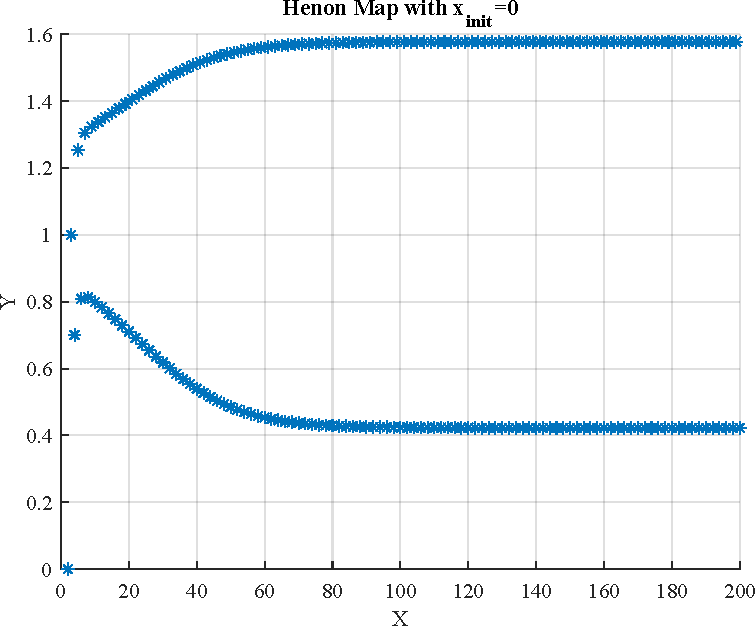
\includegraphics[width=\textwidth]{../Problem 3/prob3_x_init_0.pdf}
		\caption{}
	\end{subfigure}
	\hspace{1mm}
	\begin{subfigure}{.47\textwidth}
		\centering
		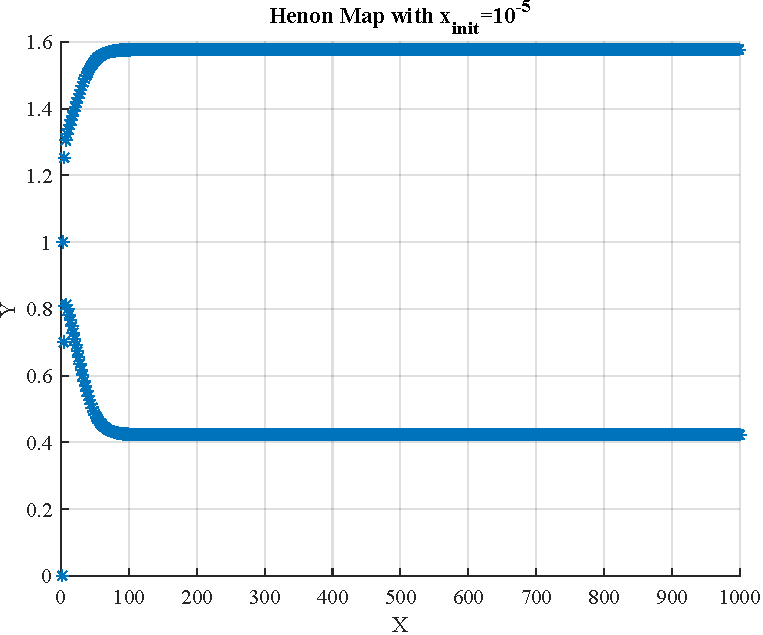
\includegraphics[width=\textwidth]{../Problem 3/prob3_x_init_1e-5.pdf}
		\caption{}
	\end{subfigure}
	\caption{Trajectories of Henon map's sequence with (a,b) = (0.3, 0.4)}
	\label{fig:prob3_x_init}
\end{figure}
From the produced plots, this system with parameters (0.3, 0.4) is periodic after converging.

\subsection{Multiple a values}
Figure~\ref{fig:prob3_multiple_a} shows output of the sequence for different values of $a$ and $b=0$. When $a \le 0.6$, the output swings for a bit and then stabilizes to a fixed number, with that number decreasing while $a$ approaches $0.6$.


\begin{figure}[htpb]
	\centering
	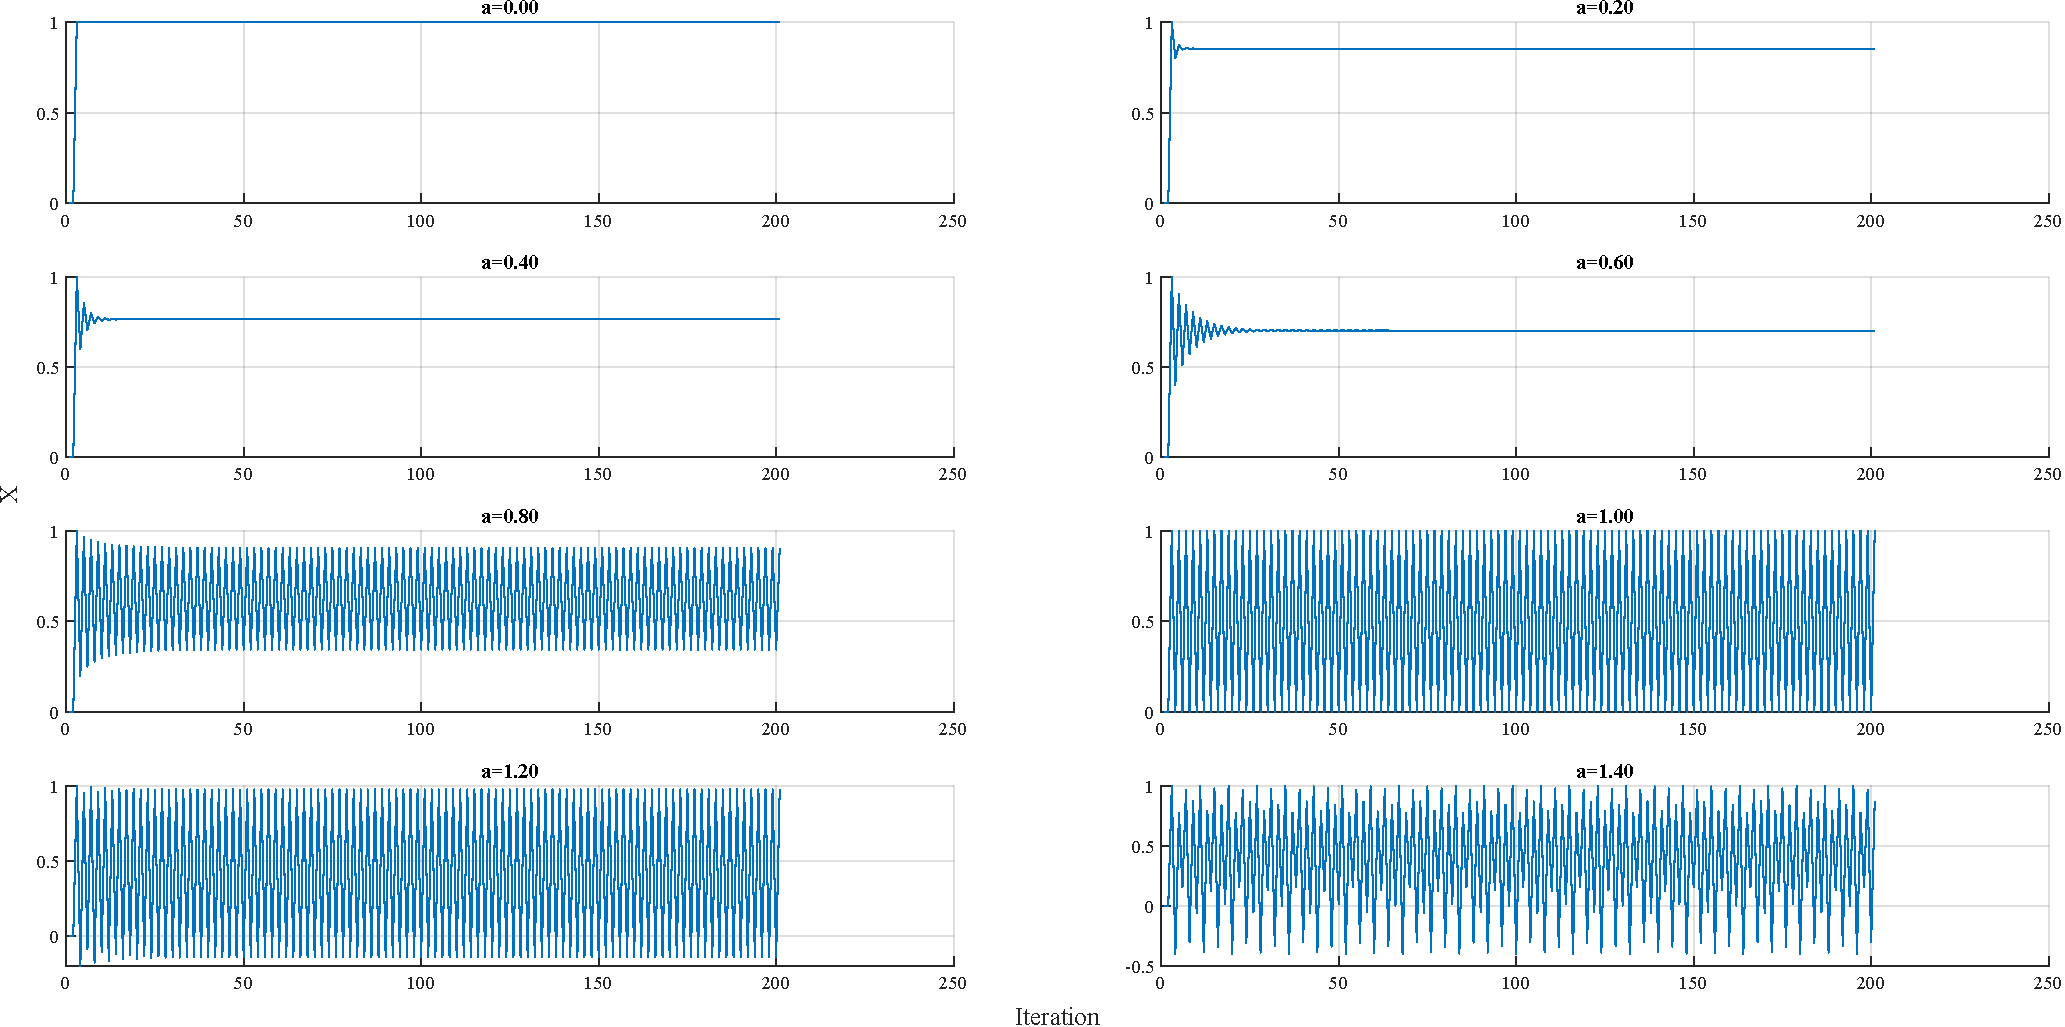
\includegraphics[width=\textwidth]{../Problem 3/prob3_(a)_multiple_a_b_0.pdf}
	\caption{Sequence output for different $a$ and $b=0$}
	\label{fig:prob3_multiple_a}
\end{figure}

When $a \ge 0.8$, output starts to oscillate. As $a$ approaches $1$, the oscillation's amplitude is getting bigger until it reaches value $1$.
After $a$ surpasses $1$, the oscillation starts to break down, as shown in the last two sub-figures. The greater $a$, the greater the disturbance on the oscillation thus chaos is created.

\subsection{Multiple initial x values}

Figure~\ref{fig:prob3_multiple_x_multiple_b} shows the trajectory of sequences with different $x_{init}$ and $b$, with $a = c, \ \text{where} \ c = 0.3$ from previous question.
Inspecting this figure, we can understand some things about those parameters and what they affect on the system, as even with $b=0$, the system performs a damped oscillation for the first 50 (at most) $x_i$.
For a given $x_{init}$ (ie. $0$), increasing $b$ increases the amplitude of oscillation as well as the overshoot percentage (if we see it as an system response).

\textit{\footnotesize PS: Overshoot \% is the percentage of system's maximum value that surpasses its steady-state value over the latter.}


\begin{figure}[htpb]
	\centering
	\begin{subfigure}{0.47\textwidth}
		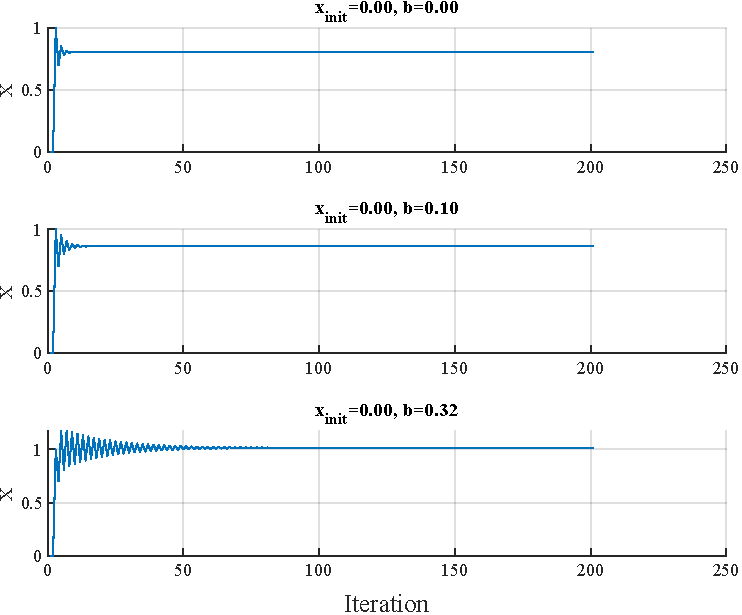
\includegraphics[width=\textwidth]{../Problem 3/prob3_(b)_x_init_0.00.pdf}
		\caption{}
	\end{subfigure}
	\begin{subfigure}{0.47\textwidth}
		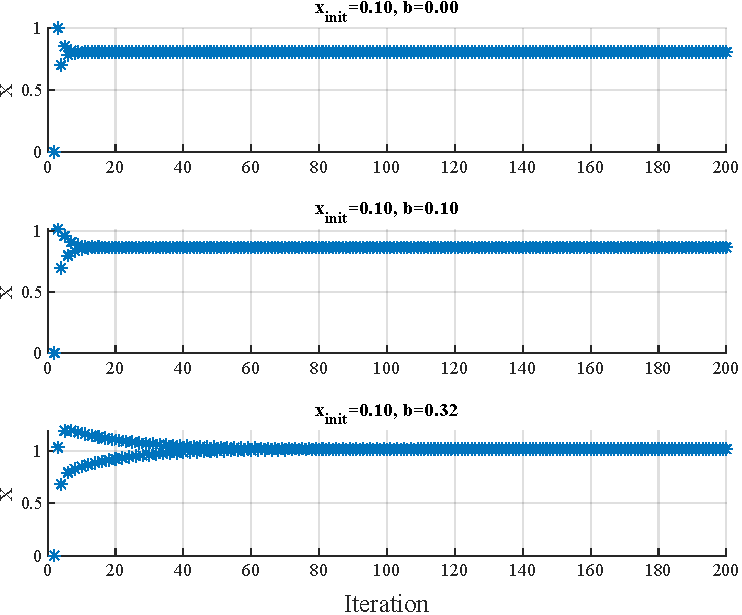
\includegraphics[width=\textwidth]{../Problem 3/prob3_(b)_x_init_0.10.pdf}
		\caption{}
	\end{subfigure}\\[4mm]
	\begin{subfigure}{0.47\textwidth}
		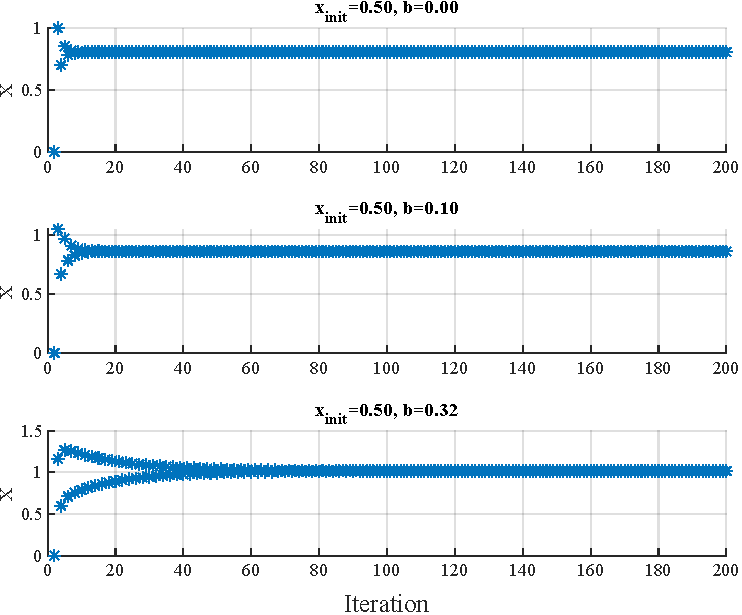
\includegraphics[width=\textwidth]{../Problem 3/prob3_(b)_x_init_0.50.pdf}
		\caption{}
	\end{subfigure}
	\begin{subfigure}{0.47\textwidth}
		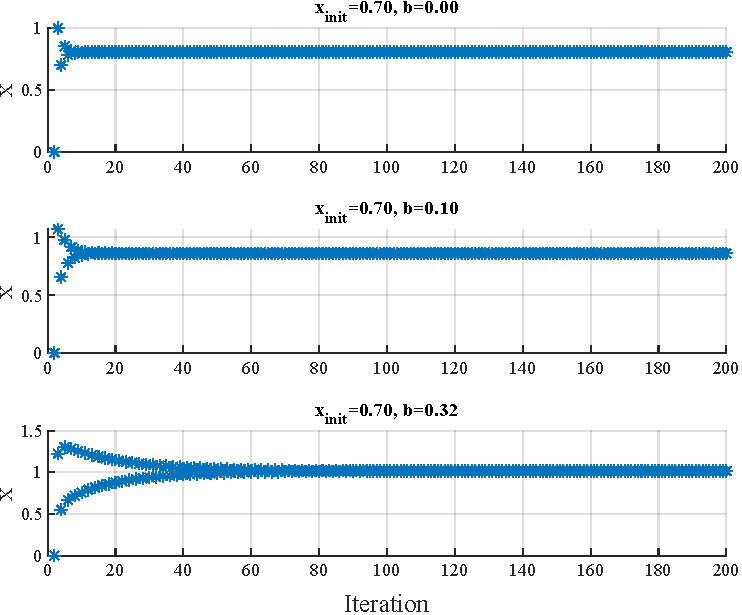
\includegraphics[width=\textwidth]{../Problem 3/prob3_(b)_x_init_0.70.pdf}
		\caption{}
	\end{subfigure}\\[4mm]
	\begin{subfigure}{0.47\textwidth}
		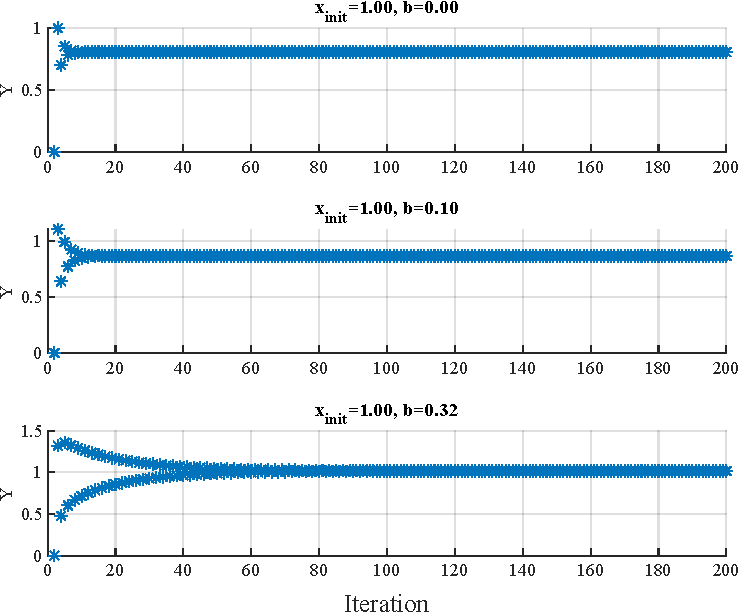
\includegraphics[width=\textwidth]{../Problem 3/prob3_(b)_x_init_1.00.pdf}
		\caption{}
	\end{subfigure}
	\caption{}
	\label{fig:prob3_multiple_x_multiple_b}
\end{figure}

\subsection{(a,b) = (0.3675, 0.3)}

By setting these values to the system, we observe that the sequence starts to oscillate with a very high frequency. As the sequence progresses, the observed oscillation's amplitude dampens and settles around a fixed number, whilst still oscillating.

\begin{figure}[htpb]
	\centering
	\begin{subfigure}{0.4\textwidth}
		\centering
		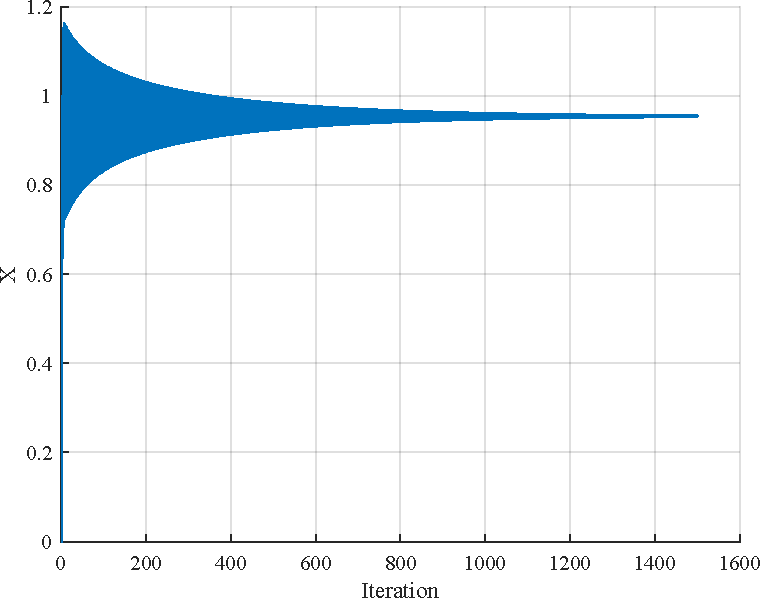
\includegraphics[width=\textwidth]{../Problem 3/prob3_(c)_a_0.365_b_0.3.pdf}
		\caption{Normal trajectory}
	\end{subfigure}
	\begin{subfigure}{0.4\textwidth}
		\centering
		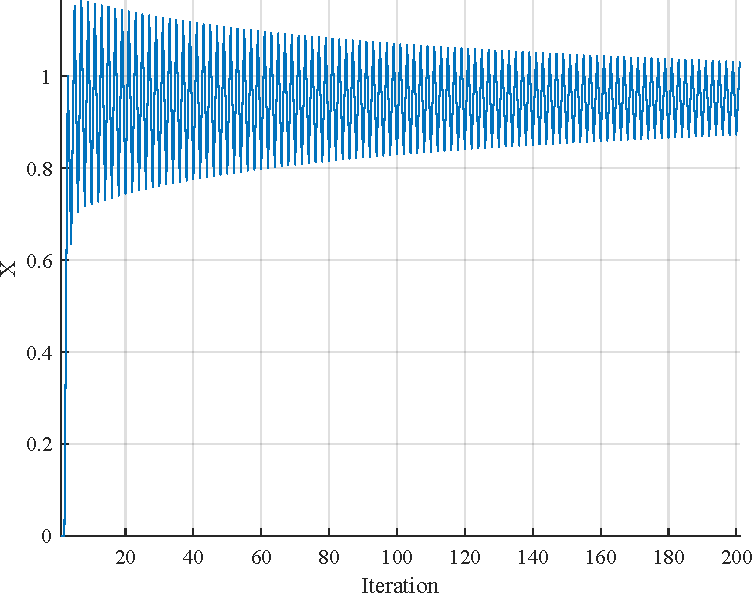
\includegraphics[width=\textwidth]{../Problem 3/prob3_(c)_a_0.365_b_0.3_zoomed.pdf}
		\caption{Zoomed in}
	\end{subfigure}
	\caption{Sequence's trajectory with (0.3675, 0.3)}
\end{figure}

\subsection{Multiple a values}

By changing $a$ parameter, we can spot and characterize system's output. Observing figure~\ref{fig:prob3_d_multiple_a}, we understand that increasing the parameter's value increases oscillation duration. At first, (when $a$ is smaller to $b$), the system oscillates for a bit and then dampens around a fixed number. But as $a$ approaches $b$, oscillation duration gets bigger until the moment where $a=b$.
From this value and over, oscillation lasts for all $x_i$. As $a$ increases beyond $b$, the oscillations begin to deteriorate, and beyond a certain point of a, chaos ensues.
\begin{figure}[htbp]
	\centering
	\begin{subfigure}{0.3\textwidth}
		\centering
		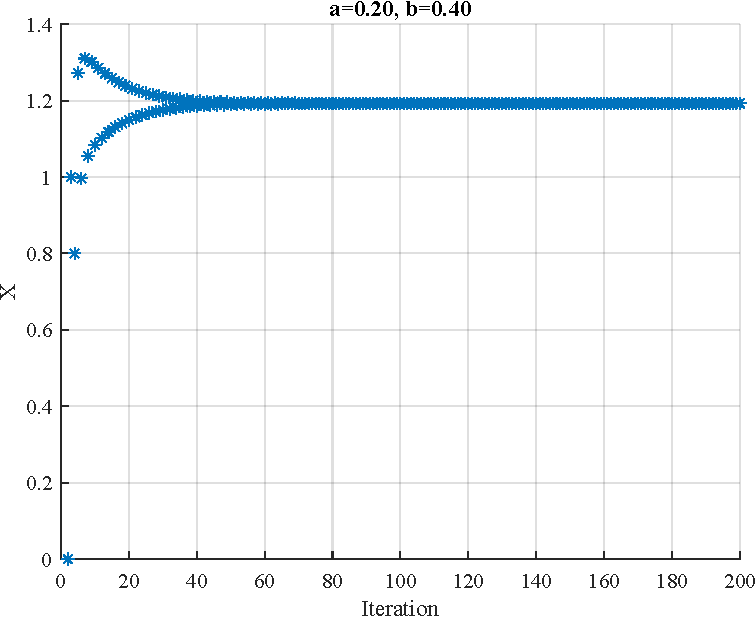
\includegraphics[width=\textwidth]{../Problem 3/prob3_(d)_a_0.20_b_0.40.pdf}
		\caption{}
	\end{subfigure}
	\begin{subfigure}{0.3\textwidth}
		\centering
		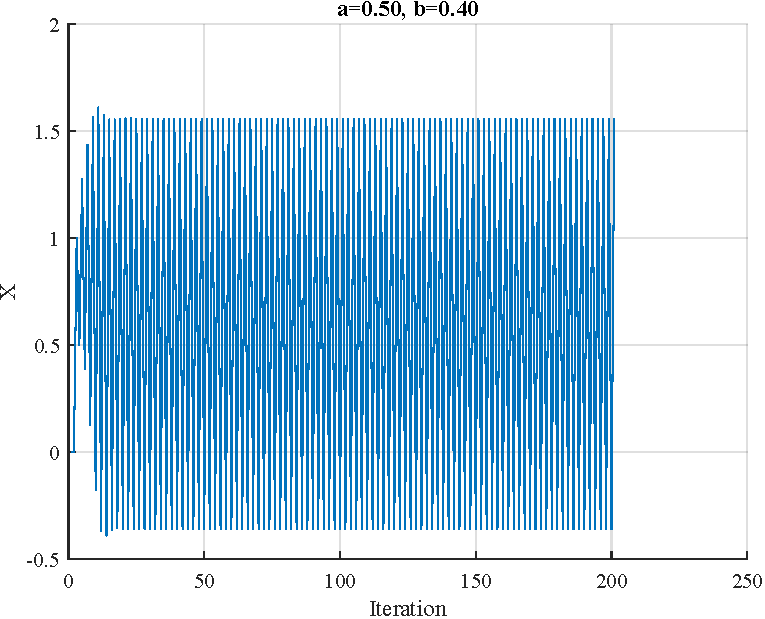
\includegraphics[width=\textwidth]{../Problem 3/prob3_(d)_a_0.50_b_0.40.pdf}
		\caption{}
	\end{subfigure}
	\begin{subfigure}{0.3\textwidth}
		\centering
		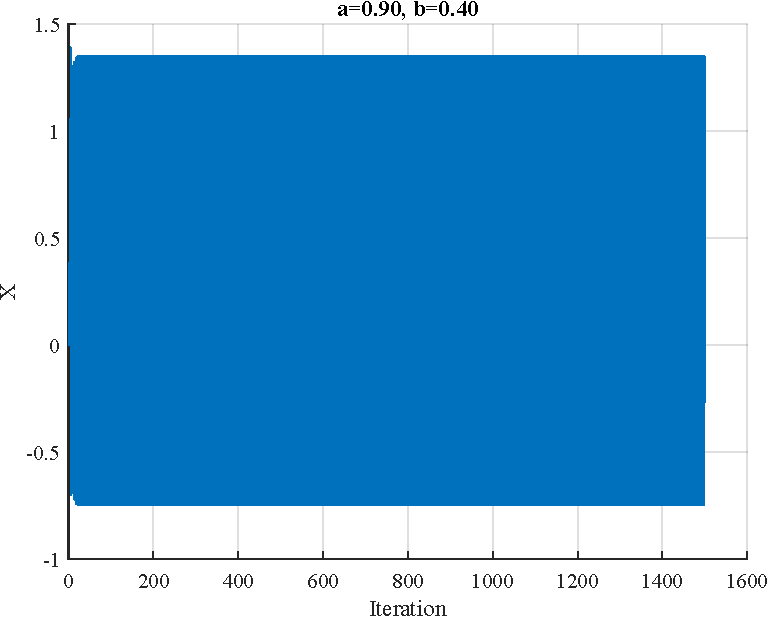
\includegraphics[width=\textwidth]{../Problem 3/prob3_(d)_a_0.90_b_0.40.pdf}
		\caption{}
	\end{subfigure}
	\caption{}
	\label{fig:prob3_d_multiple_a}
\end{figure}
